\section{Useful Properties of Kronecker-Delta and Levi-Civita}
\begin{theorem}
	\begin{equation}
		\label{eq: levi-kronecker-property-1}
		\epsilon_{pqr}\epsilon_{ruv} = (\delta_{pu}\delta_{qv} - \delta_{pv}\delta_{qu})
	\end{equation}
\end{theorem}
\begin{note}
	These are useful identity/trick to remember (remeber the use of {\bf Einstein's Notation})
	$$\delta_{aa} = \delta_{11} + \delta_{22} + \delta_{33} = 3$$
	\\
	\begin{equation*}
		\delta_{ab}\delta_{bc}=\delta_{a1}\delta_{1c} + \delta_{a2}\delta_{2c} + \delta_{a3}\delta_{3c}
		= \begin{cases}
			1 & \text{if } a = c    \\
			0 & \text{if } a \neq c
		\end{cases}
		\ \ \ = \delta_{ac}
	\end{equation*}
\end{note}


\section{Triple Vector Product}
\begin{theorem}[Triple Vector Product]
	Let $\underline{a}, \underline{b}, \underline{c} \in \mathbb{E}^3$
	\begin{equation}
		\label{eq: triple-vector-product}
		\underline{a} \times (\underline{b} \times \underline{c}) = \underline{b}(\underline{a} \cdot \underline{c}) - \underline{c}(\underline{a} \cdot \underline{b})
	\end{equation}
\end{theorem}
\begin{proof}
	Taking three vectors $\underline{a}, \underline{b} \text{ and } \underline{c}$, we {\em calculate} the \textbf{pth component} first:
	\begin{align*}
		[\underline{a} \times (\underline{b} \times \underline{c})]_{p} & = \epsilon_{pqr}\ a_{q}(\underline{b} \times \underline{c})_{r} \\ \\
		                                                                & = \epsilon_{pqr}\ a_{q} \ \epsilon_{ruv}\ b_{u}\ c_{v}
	\end{align*}
	using identity \ref{eq: levi-kronecker-property-1}, we get
	\begin{align*}
		[\underline{a} \times (\underline{b} \times \underline{c})]_{p} & = (\delta_{pu}\delta_{qv} - \delta_{pv}\delta_{qu})a_{q}b_{u}c_{v}
	\end{align*}
	Use the explanation below for completion
\end{proof}

\begin{figure}[H]
	\centering
	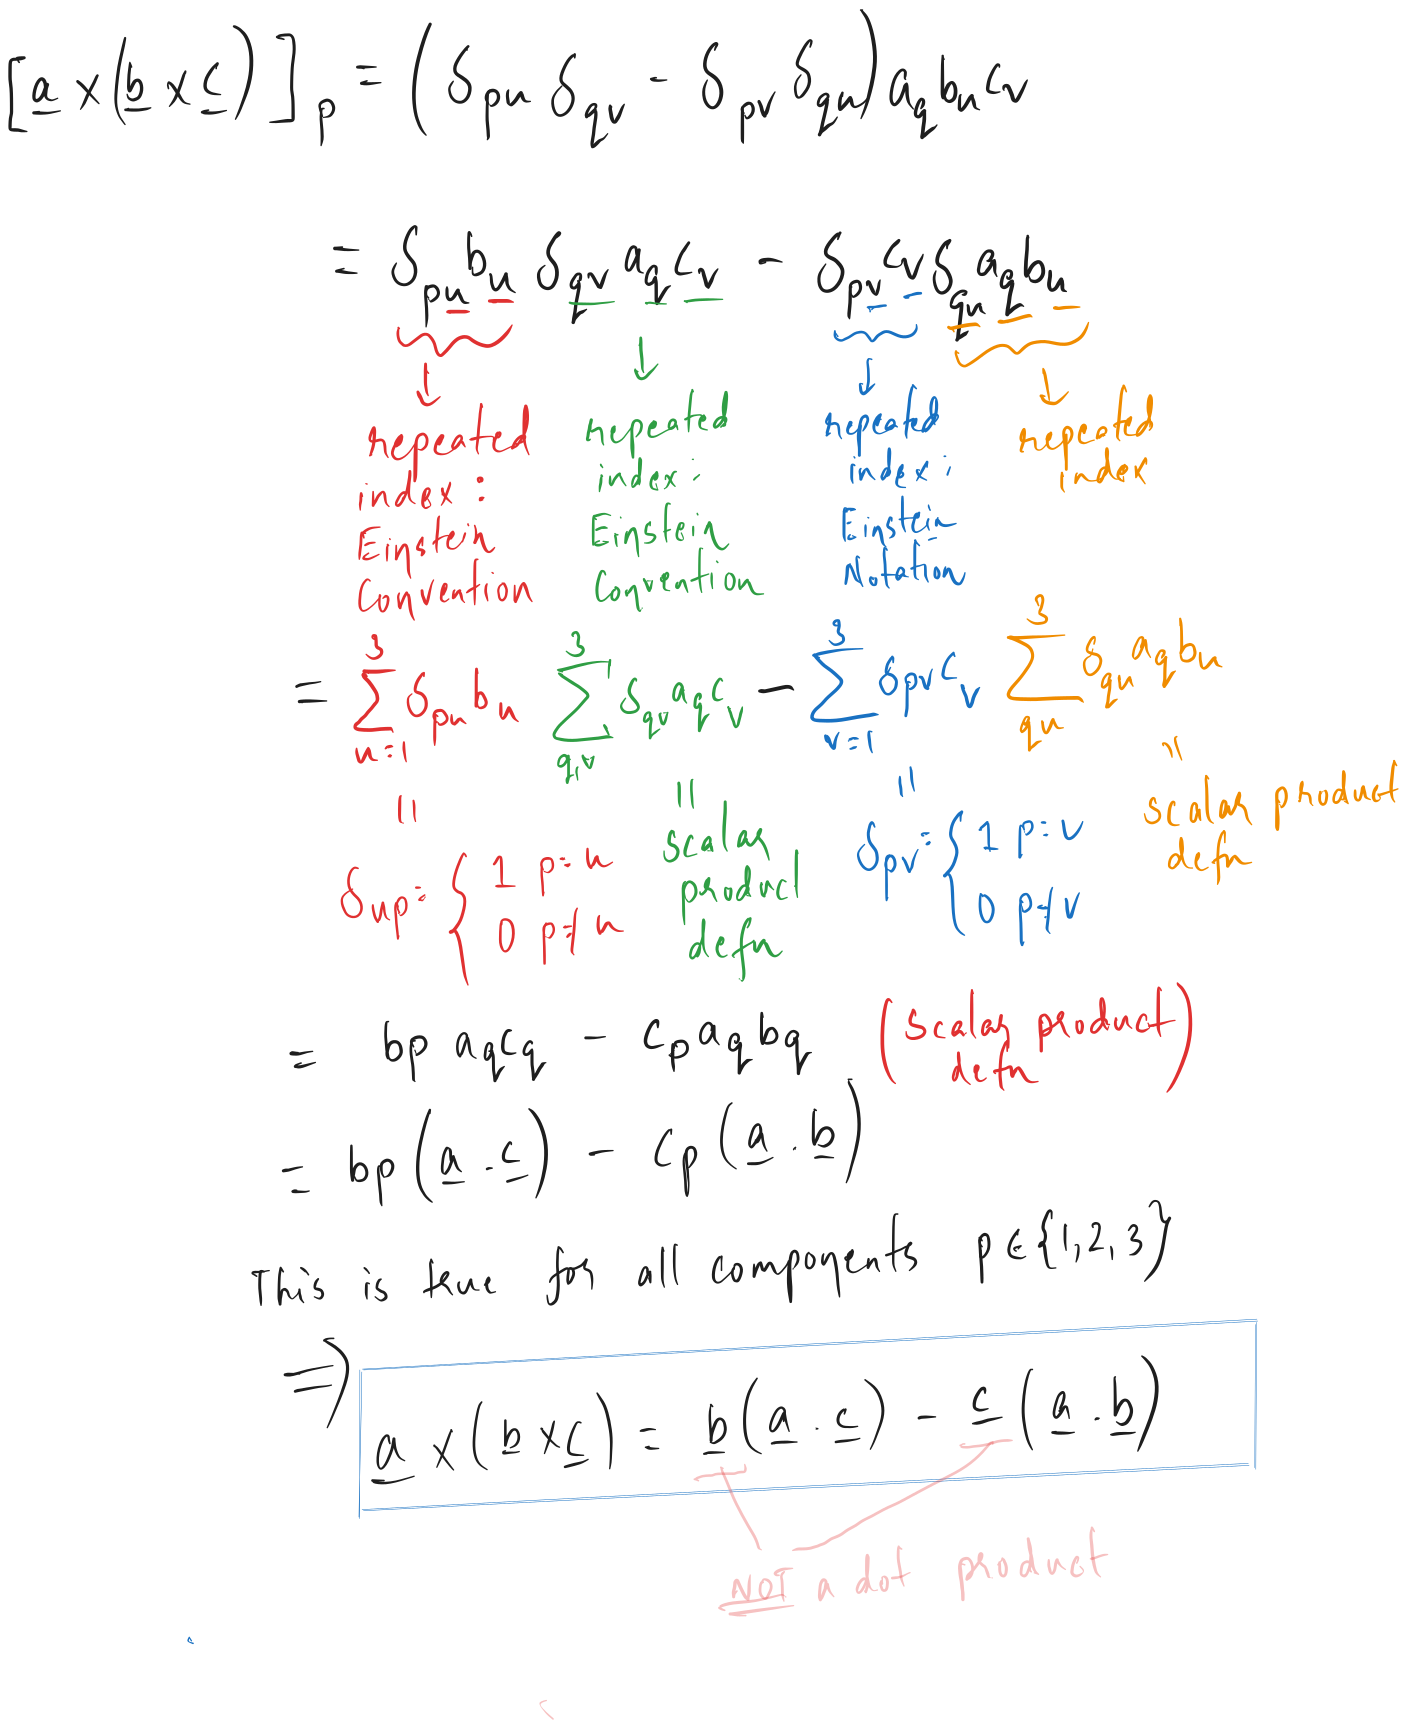
\includegraphics[scale=0.35]{triple-vector-product-proof.png}
	\caption{Triple Vector Product Proof}
	\label{fig:figure-triple-vector-product-proof}
\end{figure}

\clearpage
